\documentclass[9pt,twocolumn,twoside,]{pnas-new}

% Use the lineno option to display guide line numbers if required.
% Note that the use of elements such as single-column equations
% may affect the guide line number alignment.


\usepackage[T1]{fontenc}
\usepackage[utf8]{inputenc}

% tightlist command for lists without linebreak
\providecommand{\tightlist}{%
  \setlength{\itemsep}{0pt}\setlength{\parskip}{0pt}}



\providecommand{\pandocbounded}[1]{#1}
\usepackage{booktabs}
\usepackage{float}
\usepackage{graphicx}
\usepackage{amsmath}
\usepackage{amsfonts}
\usepackage{amssymb}
\usepackage{bbm}
\usepackage{algorithm}
\usepackage{algpseudocode}
\DeclareMathOperator*{\argmin}{argmin}
\DeclareMathOperator*{\argmax}{argmax}
\DeclareMathOperator\diag{diag}
\renewcommand{\algorithmicrequire}{\textbf{Input:}}
\renewcommand{\algorithmicensure}{\textbf{Output:}}

\templatetype{pnasresearcharticle}  % Choose template

\title{Survival driven deconvolution (deSurv) reveals prognostic and
interpretable tumor gene signatures}

\author[a,1,2]{Amber Young}
\author[b]{Alisa}
\author[a]{Didong}
\author[a,c]{Naim}

  \affil[a]{University of North Carolina at Chapel Hill, Department,
Street, City, State, Zip}
  \affil[b]{Another University Department, Street, City, State, Zip}


% Please give the surname of the lead author for the running footer
\leadauthor{Anonymous}

% Please add here a significance statement to explain the relevance of your work
\significancestatement{Authors must submit a 120-word maximum statement
about the significance of their research paper written at a level
understandable to an undergraduate educated scientist outside their
field of speciality. The primary goal of the Significance Statement is
to explain the relevance of the work in broad context to a broad
readership. The Significance Statement appears in the paper itself and
is required for all research papers.}


\authorcontributions{Please provide details of author contributions
here.}

\authordeclaration{Please declare any conflict of interest here.}


\correspondingauthor{\textsuperscript{2} To whom correspondence should
be addressed. E-mail:
\href{mailto:bob@email.com}{\nolinkurl{bob@email.com}}}

% Keywords are not mandatory, but authors are strongly encouraged to provide them. If provided, please include two to five keywords, separated by the pipe symbol, e.g:
 \keywords{  one |  two |  optional |  optional |  optional  } 

\begin{abstract}
Molecular subtyping in cancer is an ongoing problem that relies on the
identification of robust and replicable gene signatures. While
transcriptomic profiling has revealed recurrent gene expression patterns
in various types of cancer, the prognostic value of these signatures is
typically evaluated in retrospect. This is due to the reliance on
unsupervised learning methods for identifying cell-type-specific signals
and clustering patients into molecular subtypes. Here we present a
Survival-driven Deconvolution tool (deSurv) that integrates bulk
RNA-sequencing data with patient survival information to identify
cell-type-enriched gene signatures associated with prognosis. Applying
deSurv to various cohorts in pancreatic, bladder, and colorectal cancer,
we uncover previously unrecognized gene signatures linked to tumor,
stromal, and immune compartments, including … Several identified
signatures exhibit consistent prognostic value across cohorts and cancer
types and demonstrate potential as therapeutic targets or biomarkers.
Our approach highlights the value of using patient outcomes during gene
signature discovery.
\end{abstract}

\dates{This manuscript was compiled on \today}
\doi{\url{www.pnas.org/cgi/doi/10.1073/pnas.XXXXXXXXXX}}

\begin{document}

% Optional adjustment to line up main text (after abstract) of first page with line numbers, when using both lineno and twocolumn options.
% You should only change this length when you've finalised the article contents.
\verticaladjustment{-2pt}



\maketitle
\thispagestyle{firststyle}
\ifthenelse{\boolean{shortarticle}}{\ifthenelse{\boolean{singlecolumn}}{\abscontentformatted}{\abscontent}}{}

% If your first paragraph (i.e. with the \dropcap) contains a list environment (quote, quotation, theorem, definition, enumerate, itemize...), the line after the list may have some extra indentation. If this is the case, add \parshape=0 to the end of the list environment.

\acknow{Please include your acknowledgments here, set in a single
paragraph. Please do not include any acknowledgments in the Supporting
Information, or anywhere else in the manuscript.}

Molecular subtyping has become a cornerstone of precision oncology,
enabling the stratification of cancer patients based on distinct gene
expression patterns {[}Kandoth et al., 2013; Hoadley et al., 2018{]}.
This stratification informs prognosis, guides therapeutic decisions, and
enhances our understanding of tumor biology.

Nonnegative matrix factorization (NMF), first introduced by Lee and
Seung for image decomposition {[}Lee \& Seung, 1999{]}, has become a
widely used technique for dimensionality reduction and feature learning.
Unlike other matrix factorization approaches, the nonnegativity
constraint in NMF yields an additive, parts-based representation that
facilitates interpretability of latent factors. These properties have
motivated extensive methodological development, leading to extensions
that incorporate domain knowledge, structural constraints, or
supervision. Examples include sparsity-regularized formulations
{[}Hoyer, 2004{]}, graph-regularized NMF {[}Cai et al., 2008{]}, and
more recent supervised formulations such as NMFProfiler for multi-omics
integration and clinical stratification {[}Mercadié et al., 2025{]}, as
well as Bayesian multi-study NMF frameworks for mutational signatures
{[}Grabski et al., 2025{]}. Collectively, these frameworks highlight the
flexibility of NMF as a foundation for problem-specific decompositions.

High-throughput cancer transcriptomic datasets pose unique challenges
for matrix factorization: they are high-dimensional, reflect mixtures of
tumor and stromal populations, and are increasingly paired with censored
survival outcomes. Standard applications of NMF in this domain typically
follow a two-stage procedure---first identifying latent factors in an
unsupervised manner, then testing their association with overall
survival {[}Brunet et al., 2004; Bailey et al., 2016{]}. This
retrospective strategy can uncover biologically meaningful patterns, but
it does not optimize the decomposition with respect to patient outcomes,
often yielding factors dominated by non-prognostic variation such as
tumor purity, stromal admixture, or batch effects {[}Aran et al., 2017;
Thorsson et al., 2018{]}. Although supervised and discriminant variants
of NMF have been explored {[}Tran et al., 2024{]}, and some recent works
have coupled factorization with survival analysis (e.g., Learning
Individual Survival Models from PanCancer Whole Transcriptomes {[}Kumar
et al., 2023{]}; CoxNTF {[}Fogel et al., 2025{]}), these approaches
either treat survival as a downstream predictor or rely on tensor
factorizations not tailored to high-dimensional gene expression data.

To address this gap, we introduce deSurv, a survival-driven
deconvolution framework that integrates NMF with the Cox proportional
hazards model {[}Cox, 1972{]}. deSurv directly incorporates survival
information during factorization, producing interpretable, prognostic
components while providing principled model selection criteria and
regularization for high-dimensional stability {[}Tibshirani, 1997{]}.
Implemented in a scalable pipeline for large cohorts, deSurv improves
survival prediction relative to conventional unsupervised NMF while
retaining interpretability. These results establish deSurv as a general
framework for outcome-driven molecular subtyping across cancer types.

\section*{Materials and methods}\label{materials-and-methods}
\addcontentsline{toc}{section}{Materials and methods}

\subsection*{NMF}\label{nmf}
\addcontentsline{toc}{subsection}{NMF}

Let \(X \in R^{p \times n}_{\geq 0}\) denote a nonnegative gene
expression matrix of \(p\) features (genes) across \(n\) subjects. The
goal of NMF is to approximate \(X\) as the product of two low-rank,
nonnegative matrices \begin{equation}
X \approx WH,
\end{equation} where \(W \in R^{p \times k}_{\geq 0}\) contains the gene
weights (or ``metagenes''), and \(H \in R^{k \times n}_{\geq 0}\)
contains the factor scores for each subject. The number of latent
factors \(k\) determines the dimensionality of the shared low-rank
representation. The NMF loss is defined as the residual sum of squares.

\begin{equation}\label{nmf_loss}
    \mathcal{L}(W,H)_{NMF} = ||X - WH||^2_F.
\end{equation}

\subsection*{Cox partial likelihood}\label{cox-partial-likelihood}
\addcontentsline{toc}{subsection}{Cox partial likelihood}

To incorporate survival outcomes, let \(T_i\) denote the event time and
\(C_i\) the censoring time for subject \(i\). The observed time is
\(y_i = \min(T_i,C_i)\), and the event indicator is \(\delta_i\). Given
that \(W\) is shared across datasets, we define a lower dimensional
transformation of the data: \begin{equation}
Z=X^TW \in R^{n \times k},
\end{equation} where each row \(Z_i^T\) represents the factor scores for
subject \(i\). These scores serve as covariates in a Cox proportional
hazards model: \begin{equation}
h_i(t) = h_0(t)\exp(Z_i^T\beta),
\end{equation} where \(h_0(t)\) is the baseline hazard and
\(\beta \in R^k\) are the factor specific coefficients. The Cox log
partial likelihood is then \begin{equation}\label{loglik}
  \ell(W,\beta) = \sum_{i=1}^n \delta_i \left[Z_i^T\beta - \log\left(\sum_{j:y_j \geq y_i} \exp \left(Z_j^T\beta\right) \right)\right].
\end{equation} Maximizing this quantity \ldots{}

\subsection*{DeSurv}\label{desurv}
\addcontentsline{toc}{subsection}{DeSurv}

Building on the definitions above, DeSurv combines the unsupervised NMF
reconstruction loss and the supervised Cox partial likelihood into a
single joint objective. The combined loss function is

\begin{equation}\label{loss}
    \mathcal{L}(W,H,\beta) = (1-\alpha) \mathcal{L}(W,H)_{NMF} - \alpha \mathcal{L}(W,\beta)_{cox},
\end{equation}

where \(\mathcal{L}_{cox}(W,\beta)\) is the elastic net penalized log
partial likelihood: \begin{equation}\label{pen_loglik}
  \mathcal{L}_{cox}(W,\beta) = \ell(W,\beta) + \lambda(\xi||\beta||_1 + \frac{(1-\xi)}{2} ||\beta||^2_2),
\end{equation}

where \(\lambda\) represents the penalty weight and \(\xi\) is the
balance parameter between the L1 and L2 penalty terms.

The hyperparameter \(\alpha \in [0,1]\) controls the relative
contribution of each component:

\begin{itemize}
\item $\alpha=0$ recovers standard NMF, focusing purely on reconstruction;
\item $\alpha=1$ corresponds to a fully supervised Cox model in the low-dimensional space $Z=X^TW$
\end{itemize}

Intermediate values of \(\alpha\) encourage discovery of latent
molecular programs that are both biologically coherent and
prognostically informative.

\subsection*{Update Rules}\label{update-rules}
\addcontentsline{toc}{subsection}{Update Rules}

DeSurv is optimized using an alternating minimization scheme (Algorithm
\ref{deSurv}) that iteratively updates \(W\), \(H\), and \(\beta\) until
convergence. The sub-problems for \(H\) and \(\beta\) are convex in the
corresponding parameter conditional on the others.

\begin{algorithm}
\caption{DeSurv algorithm}\label{deSurv}
    \begin{algorithmic}[1]
        \Require $X \in \mathbb{R}_{\geq 0}^{p \times n}$, $y \in \mathbb{R}^n_{\geq 0}$, $\delta \in \mathbb{R}_{0,1}^{n}$, $W^{(0)}$, $H^{(0)}$, $\beta^{(0)}$, $tol$, $maxit$
        \State $eps = \infty$
        \State $iter = 0$
        \State $loss = 0$
        \While{$eps < tol$ \textbf{and} $iter < maxit$}
            \State $W^{(iter)} = \mathop{\mathrm{argmin}}_{W \geq 0} \mathcal{L}(W^{(iter-1)},H^{(iter-1)},\beta^{(iter-1)})$
            \State $H = \mathop{\mathrm{argmin}}_{H \geq 0} \mathcal{L}(W^{(iter)},H^{(iter-1)},\beta^{(iter-1)})$
            \State $\beta = \mathop{\mathrm{argmin}}_{\beta} \mathcal{L}(W^{(iter)},H^{(iter)},\beta^{(iter-1)})$
            \State $lossNew = \mathcal{L}(W^{(iter)},H^{(iter)},\beta^{(iter)})$
            \State $eps = |lossNew - loss|/loss$
            \State $loss = lossNew$
            \State $iter = iter + 1$
        \EndWhile
        \Return $W$,$H$,$\beta$
    \end{algorithmic}
\end{algorithm}

\subsubsection*{\texorpdfstring{Update for
\(H\)}{Update for H}}\label{update-for-h}
\addcontentsline{toc}{subsubsection}{Update for \(H\)}

The nonnegative factor matrix \(H\) is updated using standard
multiplicative updates that guarantee nonnegativity and monotonic
decrease in reconstruction error as derived in \cite{@lee}:
\begin{equation}
\label{H_update}
    H_{ij} = H_{ij} \frac{(W^TX)_{ij}}{(W^TWH)_{ij}}.
\end{equation}

\subsubsection*{\texorpdfstring{Update for
\(\beta\)}{Update for \textbackslash beta}}\label{update-for-beta}
\addcontentsline{toc}{subsubsection}{Update for \(\beta\)}

Given \(W\), the coefficients \(\beta\) are updated by coordinate
descent using elastic-net regularization: \begin{equation}
\label{beta_update}
    \hat{\beta}_r = \frac{S(\frac{1}{n}\sum_{i=1}^n w(\tilde{\eta})_i v_{i,r} \left[ z(\tilde{\eta})_i - \sum_{j\ne r} v_{ij} \beta_j,\right], \lambda\xi)}{\frac{1}{n}\sum_{i=1}^n w(\tilde{\eta})_i v_{i,r}^2 + \lambda(1-\xi)},
\end{equation} where \(S(.,\lambda\xi)\) is the soft-thresholding
operator, \(w_i\) is blah, and \(v_{ij}\) . The parameters
\((\lambda,\xi)\) control the strength and type of regularization.

\subsubsection*{\texorpdfstring{Coupled \(W\)
update}{Coupled W update}}\label{coupled-w-update}
\addcontentsline{toc}{subsubsection}{Coupled \(W\) update}

The shared basis \(W\) is updated through a hybrid multiplicative rule
that incorporates both NMF reconstruction gradients and Cox partial
likelihood gradients. Backtracking and gradient balancing are used in
this update to ensure decrease in the overall loss and avoid one
component dominating the update. (Add citations for this here)
\begin{equation}
\label{W_update}
W^{(t+1)} = W^{(t)} \odot \max \left( \frac{\frac{(1-\alpha)}{np}XH^T + \frac{2\alpha}{N_{event}}\nabla_W\ell(W^{(t)}, \beta)}{\frac{(1-\alpha)}{np}W^{(t)}HH^T }, 0 \right)
\end{equation} The quantity \(\nabla_W\ell(W^{(t)}, \beta)\) denotes the
gradient of the Cox partial likelihood with respect to \(W\). This
update allows the survival signal to propagate into the latent factors
while preserving nonnegativity.

\subsection*{Publicly Available
Datasets}\label{publicly-available-datasets}
\addcontentsline{toc}{subsection}{Publicly Available Datasets}

We trained and validated DeSurv using seven publicly available
pancreatic ductal adenocarcinoma (PDAC) transcriptomic datasets spanning
both RNA-seq and microarray platforms. Expression data were harmonized
to gene-level matrices and transformed to transcripts per million (TPM)
where applicable. To reduce platform-specific bias, each dataset was
rank-transformed across genes within samples prior to modeling.

\begin{table*}[t]
\centering
\caption{Publicly available pancreatic ductal adenocarcinoma (PDAC) datasets used for model training and validation. Expression data were rank-transformed across genes within samples to mitigate platform- and scale-related effects.}
\label{tab:datasets}
\begin{tabular}{@{}lllll@{}}
\toprule
\textbf{Dataset} & \textbf{Platform} & \textbf{Samples (n)} & \textbf{Data type} & \textbf{Reference} \\ 
\midrule
TCGA-PAAD & RNA-seq (Illumina HiSeq) & $\sim$178 & Discovery / Training & \citep{TCGA2017} \\
CPTAC-PDAC & RNA-seq (Proteogenomic) & $\sim$138 & Validation & \citep{Clark2021} \\
Dijk \textit{et al.} & Microarray (Affymetrix) & $\sim$80 & Validation & \citep{Dijk2015} \\
Moffitt \textit{et al.} & Microarray (Affymetrix) & $\sim$84 & Validation & \citep{Moffitt2015} \\
PACA-AU (array) & Microarray (Agilent) & $\sim$269 & Validation & \citep{Bailey2016} \\
PACA-AU (RNA-seq) & RNA-seq (Illumina HiSeq) & $\sim$92 & Validation & \citep{Bailey2016} \\
Puleo \textit{et al.} & Microarray (Affymetrix) & $\sim$288 & Validation & \citep{Puleo2018} \\ 
\bottomrule
\end{tabular}
\end{table*}

\subsection*{Model Training}\label{model-training}
\addcontentsline{toc}{subsection}{Model Training}

The TCGA and CPTAC datasets were used for model training. Each dataset
was filtered to the top 2000 highly expressed and variable genes. These
gene lists were then intersected, resulting in XXX genes incorporated in
model training.

\subsection{Cross Validation}\label{cross-validation}

To identify optimal hyperparameters, we employed stratified five-fold
cross-validation based on event status. An exhaustive search was
performed across a grid of hyperparameters \(k = 2,\dots,12\),
\(\alpha \in \{0.1,0.2,\dots,0.9\}\), \(\lambda \in 10^{\{-3,...,3\}}\),
and \(\xi \in \{0,0.1,0.2,\dots,1\}\). Within each fold, models were fit
on 80\% of the data and evaluated on the held-out 20\%. Because NMF
solutions are non-unique and sensitive to initialization, each fold was
repeated with 20 random seeds for \(W\), \(H\), and \(\beta\), resulting
in a total of 100 trained models per parameter configuration of \(k\),
\(lambda\), and \(eta\). Warm-start initializations were used across
\(alpha\) to accelerate convergence.

Final hyperparameters were selected as the combination that produced
average C-index (across initializations and folds) within one standard
error of the maximum (1 s.e. rule).

\subsection*{Comparison Methods}\label{comparison-methods}
\addcontentsline{toc}{subsection}{Comparison Methods}

To benchmark the performance of DeSurv, we compared it against several
established approaches for molecular subtyping and survival prediction.
All comparison models were trained using the same discovery cohort, the
same filtered set of 1,000 highly variable genes, and the same
preprocessing steps.

\subsubsection*{Standard NMF}\label{standard-nmf}
\addcontentsline{toc}{subsubsection}{Standard NMF}

As an unsupervised baseline, we trained conventional NMF models that
minimized only the reconstruction error, corresponding to setting
\(alpha=0\) in the DeSurv formulation. For each rank
\(k \in {2,...,12}\), 100 random initializations were performed to
address non-uniqueness. The initialization with the smallest
reconstruction error for each k was selected. To select the rank, \(k\),
in the unsupervised setting, we use standard metrics including
cophenetic coefficient, dispersion, explained variance, residuals,
silhouette score, and sparseness. The resulting gene-factor matrix \(W\)
and validation data were subsequently used as input to a Cox
proportional hazards model to evaluate the prognostic value of the
unsupervised factors.

\subsubsection*{Cox Elastic Net (CoxNet)}\label{cox-elastic-net-coxnet}
\addcontentsline{toc}{subsubsection}{Cox Elastic Net (CoxNet)}

We also compared DeSurv to a standard penalized Cox regression model fit
directly to gene-level expression data with elastic net penalty.
Five-fold internal cross-validation within the training data was used to
select the penalization parameters based on the mean C-index. The final
CoxNet model served as a high-dimensional supervised baseline without
dimensionality reduction.

\subsection*{Model Validation}\label{model-validation}
\addcontentsline{toc}{subsection}{Model Validation}

The remaining 6 publicly available PDAC datasets, CPTAC, Dijk, Moffitt,
PACA microarray, PACA RNAseq, and Puleo, were used to validate our
models. The datasets were restricted to the same highly variable genes
in the TCGA dataset, and the fitted model was applied to each dataset
individually. The partial likelihood and c-index were calculated for
each dataset. Hazard ratios were reported for each factor.

\subsection*{Score based approach}\label{score-based-approach}
\addcontentsline{toc}{subsection}{Score based approach}

In a clinical setting, it may not be feasible to sequence all of the
genes required to port the full W matrix to future test sets. For this
purpose we also propose a score based method, where only the identity of
top genes for each factor must be ported to future datasets. To
construct the scores we define Wtilde as a binary matrix\ldots{} To
predict patient outcomes in future datasets, we restrict those datasets
to these g x k genes, and compute XtWtilde as linear predictor in the
survival model.

\subsection*{Top genes}\label{top-genes}
\addcontentsline{toc}{subsection}{Top genes}

For a factor \(f\) a top gene is defined as a gene that is highly
weighted in factor \(f\) while being lowly weighted in all other
factors. We define \(s_{gf}\) as the difference in weights between gene
\(g\) in factor \(f\) and the max weight across all other factors in
gene \(g\).

\begin{equation}
s_{gf} = W_{gf} - \max_{r \ne f}(W_{gr})
\end{equation}

\subsection*{Clustering}\label{clustering}
\addcontentsline{toc}{subsection}{Clustering}

\section*{Results}\label{results}
\addcontentsline{toc}{section}{Results}

\subsection{The NMF--Cox framework provides an end-to-end workflow for
prognostic
modeling}\label{the-nmfcox-framework-provides-an-end-to-end-workflow-for-prognostic-modeling}

We developed an integrated framework that combines nonnegative matrix
factorization (NMF) with Cox proportional hazards regression to identify
latent gene expression factors associated with survival. As illustrated
in Figure 1, the workflow begins with preprocessing and normalization of
RNA-seq data, followed by NMF decomposition into patient factor loadings
(\(W\)) and gene weightings (\(H\)). A Cox model is then fit using
projected covariates derived from W. The framework incorporates a
balancing parameter \(\alpha\) to control the relative influence of
reconstruction error versus survival likelihood. Model selection is
performed via cross-validation across k, penalty parameters, and
\(\alpha\), with downstream evaluation focusing on both predictive
performance and biological interpretability.

\begin{figure*}[t]

{\centering 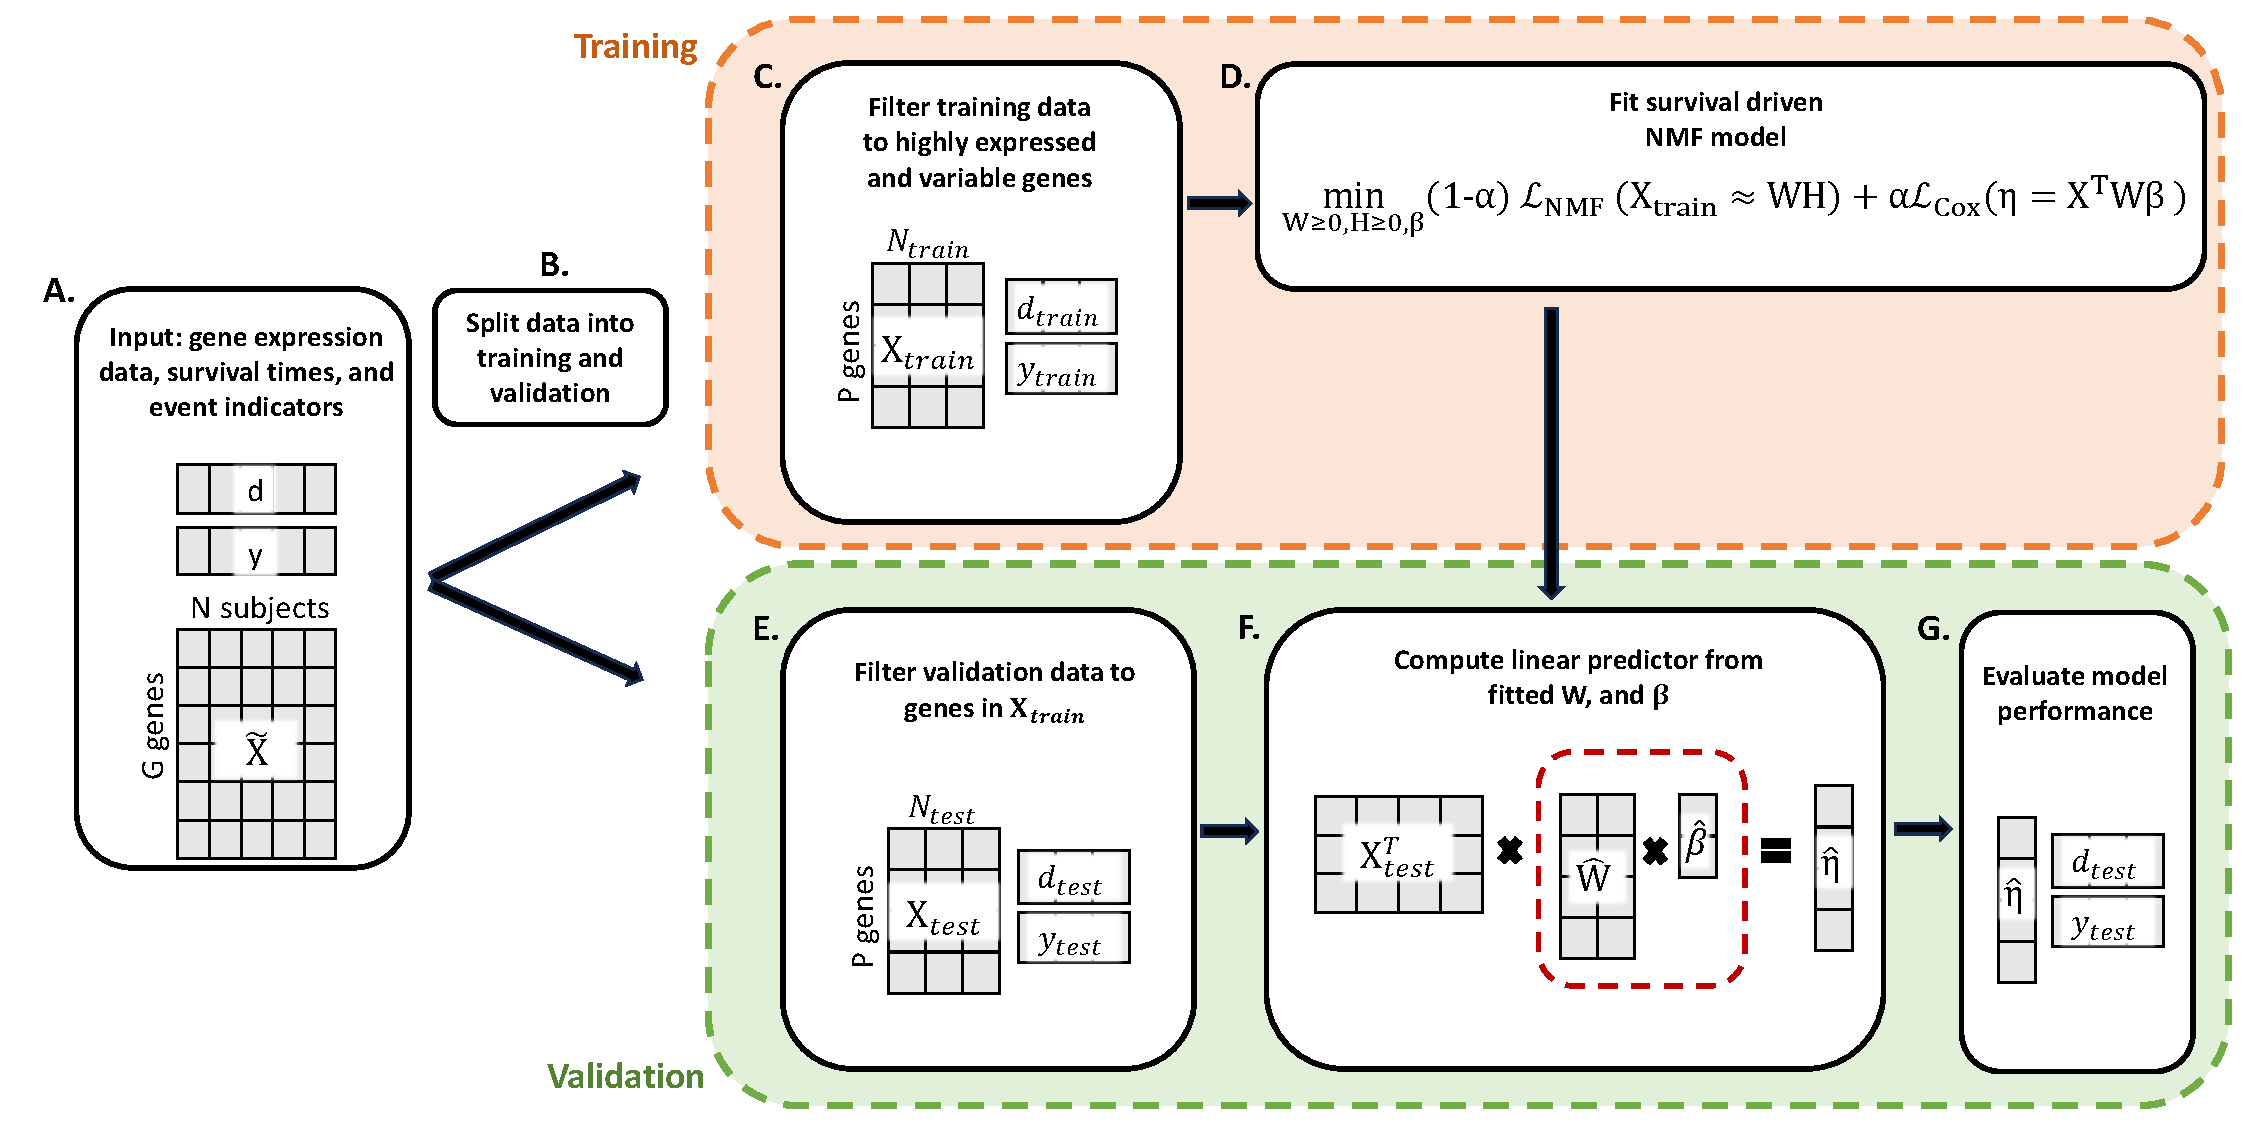
\includegraphics[width=\textwidth,height=4in]{../figures/model_schematic_with_validation} 

}

\caption{DeSurv overview}\label{fig:fig-schema}
\end{figure*}

\subsection{Cross-validation of NMF--Cox identifies parameter settings
that balance prediction and
reconstruction}\label{cross-validation-of-nmfcox-identifies-parameter-settings-that-balance-prediction-and-reconstruction}

We evaluated performance across a grid of factor ranks (k), penalties,
and values of \(\alpha\). Cross-validated C-index varied modestly across
conditions, with no consistent improvement for \(\alpha>0\). Instead,
supervised extensions altered the orientation of latent factors while
maintaining comparable discrimination. Figure @ref(fig::fig-cv)A shows a
heatmap of mean C-index across k and \(\alpha\), and @ref(fig::fig-cv)B
illustrates C-index trends across \(\alpha\) stratified by rank.

\begin{figure*}[t]

{\centering 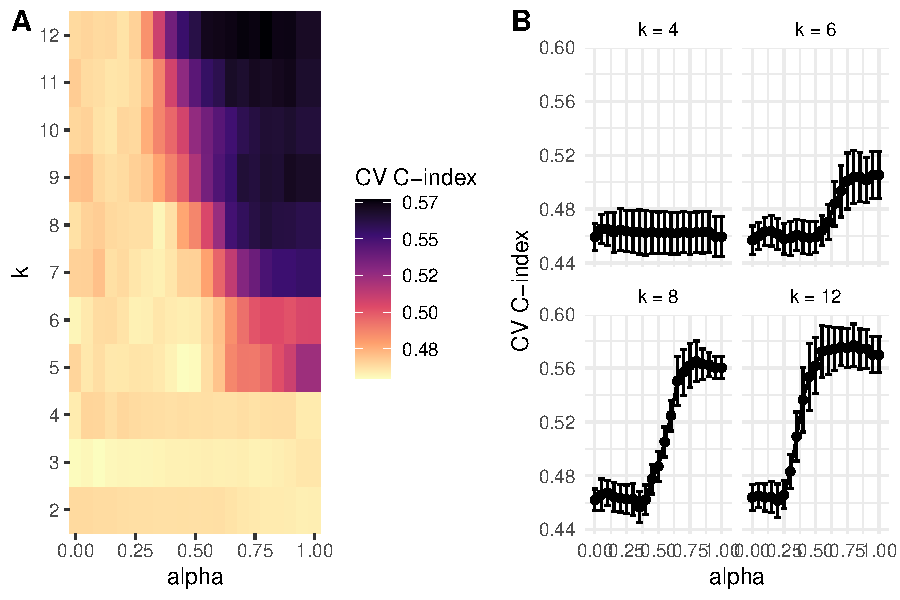
\includegraphics[width=6in,height=5.5in]{paper_files/figure-latex/fig-cv-1} 

}

\caption{A. Cross validated c-index over rank (k) with panels for various values of the trade-off parameter (alpha). B. Cross validated c-index over alpha with panels for various values of k. C. Heatmap of cross-validated c-index with columns k and rows alpha. D. Plots of various metrics used to choose k in the standard NMF setting.}\label{fig:fig-cv}
\end{figure*}

\subsection{NMF--Cox factors generalize to independent cohorts in
external
validation}\label{nmfcox-factors-generalize-to-independent-cohorts-in-external-validation}

To assess generalizability, models trained on TCGA-PAAD and CPTAC were
applied to external cohorts including PACA, Moffitt, and Puleo. Factor
exposures in validation datasets recapitulated subgroup structures
identified in training and stratified patients into groups with distinct
survival outcomes (Figure X). Factor correlation analyses (Figure X)
confirmed reproducibility of core latent dimensions, particularly those
separating basal-like and classical subtypes. Predictive accuracy in
external cohorts was comparable to cross-validation results, with
simpler models (\(k\leq 5\)) showing greater reproducibility. These
findings indicate that NMF--Cox captures transferable biological signals
across studies.

\begin{figure*}[t]

{\centering 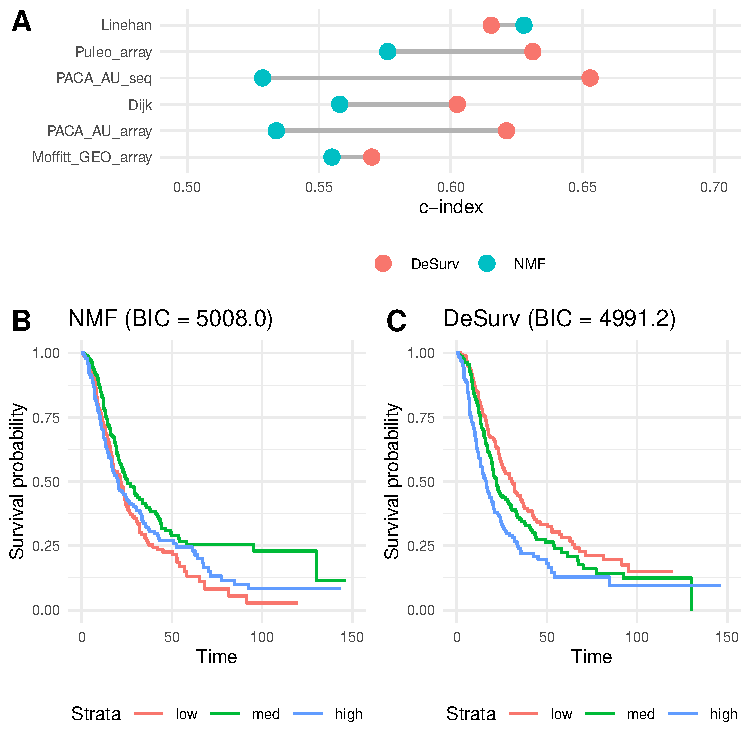
\includegraphics[width=5in,height=5in]{paper_files/figure-latex/fig-external-1} 

}

\caption{Model performance in valiation data. A. C-index for standard NMF vs DeSurv. B. Kaplan Meier curves by quantile of the linear predictor for standard NMF. C. Kaplan Meier curves by quantile of the linear predictor for DeSurv}\label{fig:fig-external}
\end{figure*}

\subsection{NMF--Cox uncovers biologically interpretable latent factors
associated with clinical
outcomes}\label{nmfcox-uncovers-biologically-interpretable-latent-factors-associated-with-clinical-outcomes}

Despite limited performance gains from supervision, the latent factors
identified by NMF--Cox exhibited strong biological interpretability. The
projected covariates, \(W^TX\), aligned with known clinical and
molecular subtypes, including basal-like versus classical subgroups in
pancreatic cancer (Figure X). Kaplan--Meier curves stratified by factor
exposures revealed significant survival differences (Figure X),
supporting the prognostic relevance of the factors. At the gene level, W
highlighted pathway-level enrichment for immune signaling, stromal
activity, and hallmark oncogenic processes. Overlap analysis (Figure X)
demonstrated consistency with external signatures, confirming that
NMF--Cox produces reproducible biological features.

\section*{Discussion}\label{discussion}
\addcontentsline{toc}{section}{Discussion}

\showmatmethods
\showacknow
\pnasbreak



% Bibliography
% \bibliography{pnas-sample}

\end{document}
